\documentclass{article}

\usepackage[latin1]{inputenc}
\usepackage{tikz}

\begin{document}
\pagestyle{empty}

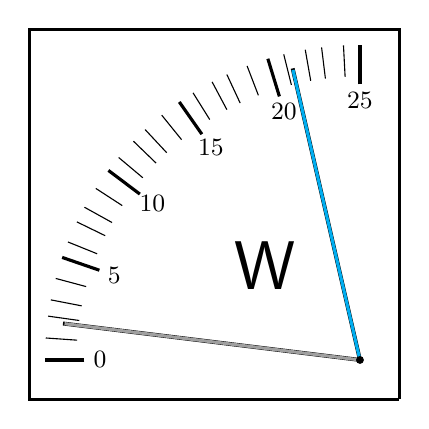
\begin{tikzpicture}
    \draw[line width=.4mm] (.5,-.5) -- (.5,4.2) -- (-4.2,4.2) -- (-4.2,-.5) -- (.5,-.5);
    \node at (-1.2,1.2) {\Huge{\textsf{W}}};
    \foreach \a in {0,3.6,...,93.6}{
        \pgfmathtruncatemacro{\b}{mod((\a)-90, 360)}
        \pgfmathtruncatemacro{\c}{\a/3.6}
        \pgfmathtruncatemacro{\d}{(mod(\c, 5))}
        \ifnum\d=0
            \node[black] at ({3.3*sin(\b)}, {3.3*cos(\b)}) {\small{\c}};
            \draw[line width=.4mm]({3.5*sin(\b)}, {3.5*cos(\b)}) -- ({4*sin(\b)}, {4*cos(\b)});
        \else
            \draw[-]({3.6*sin(\b)}, {3.6*cos(\b)}) -- ({4*sin(\b)}, {4*cos(\b)});
        \fi
    }
    \pgfmathtruncatemacro{\f}{mod((21.2*3.6)-90, 360)}
    \pgfmathtruncatemacro{\r}{mod((1.8*3.6)-90, 360)}
    \draw[color=black, line width=.5mm] (0,0) -> ({3.8*sin(\r)}, {3.8*cos(\r)});
    \draw[color=darkgray!50, line width=.4mm] (0,0) -> ({3.78*sin(\r)}, {3.78*cos(\r)});
    \draw[color=black, line width=.5mm] (0,0) -> ({3.8*sin(\f)}, {3.8*cos(\f)});
    \draw[color=cyan, line width=.4mm] (0,0) -> ({3.78*sin(\f)}, {3.78*cos(\f)});
    \fill (0,0) circle(.5mm);
\end{tikzpicture}
\\
\\
\\
\\
\\
\\
\\

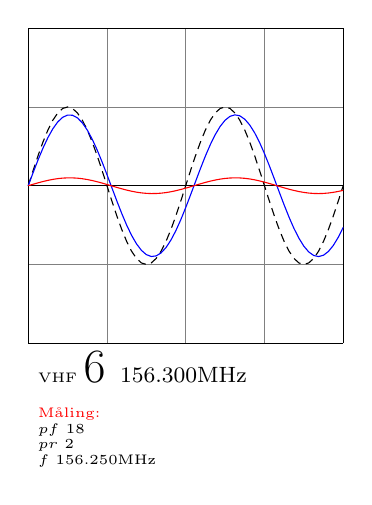
\begin{tikzpicture}[domain=0:4]
    \draw[very thin,color=gray] (0,-2) grid (4,2);
    \draw[-] (0,2) -- (4, 2);
    \draw[-] (4,2) -- (4, -2);
    \draw[-] (4,-2) -- (0, -2);
    \draw[-] (0,-2) -- (0, 2);
    \draw[-] (0,0) -- (4,0); 
    \draw[black, densely dashed, samples=65] plot (\x, {sin(pi*\x*1 r)});
    \draw[blue, samples=65] plot(\x, {(1/20)/(1/18)*sin(pi*\x*.950 r)});
    \draw[red, samples=65] plot(\x, {(1/20)/(1/2)*sin(pi*\x*.950 r)}); 
    \node[black, anchor=west] at (0,-2.3) {\tiny{VHF} \LARGE{6} \footnotesize{156.300MHz}};
    \node[red, anchor=west] at (0,-2.9) {\tiny{M\aa{}ling:}};
    \node[black, anchor=west] at (0,-3.1) {\tiny{$pf$} \tiny{18}};
    \node[black, anchor=west] at (0,-3.3) {\tiny{$pr$} \tiny{2}};
    \node[black, anchor=west] at (0,-3.5) {\tiny{$f$} \tiny{156.250MHz}};
\end{tikzpicture}


\end{document}
